

\section{Periodic solution}
\label{sec:periodic-solution}

Before turning to the methods themselves, a few concepts must be revisited.
Computing the periodic solution of a nonlinear system means searching for a
solution $\bm x$ to

\begin{equation}
    \label{eq:per_eom}
  \bm M \ddot{\bm x}(t) + \bm C \dot{\bm x}(t) + \bm K \bm x(t) +
  \bm f_{nl} \left( \bm x(t), \dot{ \bm x}(t) \right) = \bm p (t)
\end{equation}
that satisfies a periodicity condition
\begin{equation}
  \label{eq:per_condtion}
  \bm x(t+T) = \bm x(t)
\end{equation}
where $T$ is the period. This is a boundary value problem(BVP). By periodic
solution, steady state conditions are implied. Stability of the periodic
solution will also be addressed.


There are at least three ways to describe such a periodic solution.

\begin{itemize}
\item Provide initial condition $\left[\bm x_0 \dot{\bm x}_0 \right]$ and the
  period $T$. Then do time integration over $T$.
\item Use piecewise polynomial functions and the period $T$
\item Use Fourier series and the period $T$
\end{itemize}

In this section, the methods for finding the first and last representations of a
periodic solution is described. They are denoted the shooting method and
harmonic balance method respectively. The one not covered here is called
Orthogonal collocation. The shooting method is used as part of calculating NNMs
and harmonic balance is used for bifurcation analysis. Both methods could be
used for both tasks, but there are significant numerical benefits for using them
as here.


\subsection{Shooting method}
\label{sec:shooting_method}

The shooting method works by finding, in an iterative way, the initial state
$\bm z = [\bm x, \dot{\bm x}]^T$ and period $T$ that describes a periodic
motion, see \citet{nayfeh2008applied} for more details.

One start by guessing on periodic steady state(ie. initial state
and period) and then \textit{shoots} forward one period with the hope of
arriving close to the guessed initial state. The difference between the initial
and final states is used to correct the initial state, and the method
\textit{shoots} forward another period and continue until final and initial
state match.
The final state is found by integration, see appendix
\ref{chap:newmark-integration} for details on the nonlinear Newmark integration.
The corrections are done by Newton-Rahpson iterations.

The EOM \eqref{eq:per_eom} is recast into state space form. Since this method is
used for NNMs, it is recast in the undamped and unforced form.

\begin{equation}
  \label{eq:sm_state}
  \dot{\bm z} = \bm g (\bm z) =
  \begin{bmatrix}
    \dot{\bm x} \\
    -\bm M^{-1}(\bm K \bm x  + \bm f_{nl})
  \end{bmatrix}
\end{equation}


A solution $\bm z_p(t, \bm z_{p0})$ is a solution of the autonomous system eq.
\eqref{eq:sm_state} if $\bm z_p(t, \bm z_{p0}) = \bm z_p(t+T, \bm z_{p0})$ where
$T$ is the minimal period. Thus the periodic condition is

\begin{equation}
  \label{eq:sm_per_cond}
  \bm H(\bm z_{p0},T) \equiv \bm z(T, \bm z_{p0}) - \bm z_{p0} = \bm 0
\end{equation}
$\bm H$ is called the shooting function.


To make the solution $\bm z(t)$ uniquely defined, the phase must be fixed. If
$\bm z(t)$ is a solution to \eqref{eq:sm_state} then $z(t + \Delta t)$ is
geometrically the same solution in state space for any $\Delta t$. Ie. the
initial condition $\bm z_{p0}$ can be arbitrarily chosen anywhere on the
periodic solution. To prevent this, a phase condition $h(\bm z_{p0})=0$ is set
as a additional condition. Most phase conditions imposes one of the unknowns to
be set to 0, e.g. the initial displacement or velocity of a DOF(often velocity).
For NNM computations specific, other phase conditions will reduce the
computation complexity as will be mentioned in section \textbf{NNM}. See figure
\ref{fig:sm_phase} for a illustration of different phases for the periodic
solution. \textbf{ER DET ET RELEVANT PLOT? JEG SYNES TEKSTEN ER NOK.}

\begin{figure}[!ht]
  \centering
  \begin{subfigure}[b]{0.45\textwidth}
    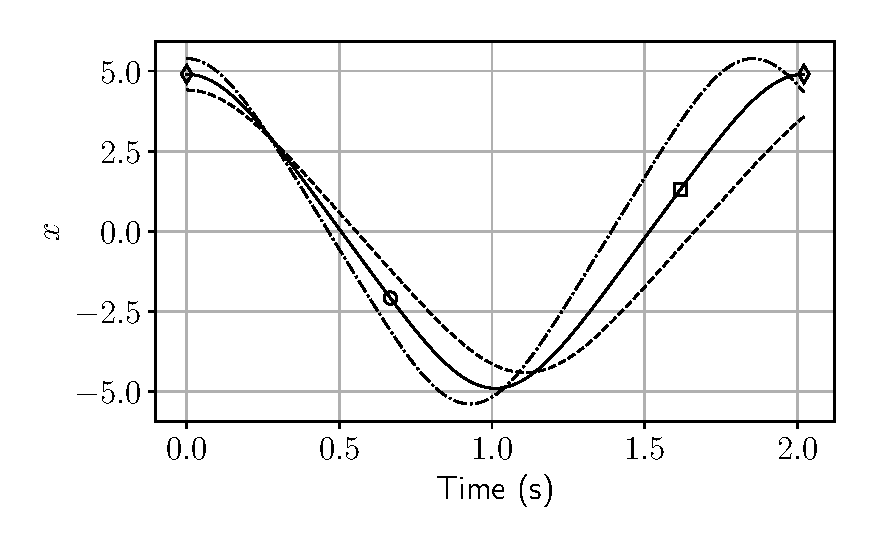
\includegraphics[width=\textwidth, height=5cm]{nnm/duff_per_time}
  \end{subfigure}
  ~
  \begin{subfigure}[b]{0.45\textwidth}
    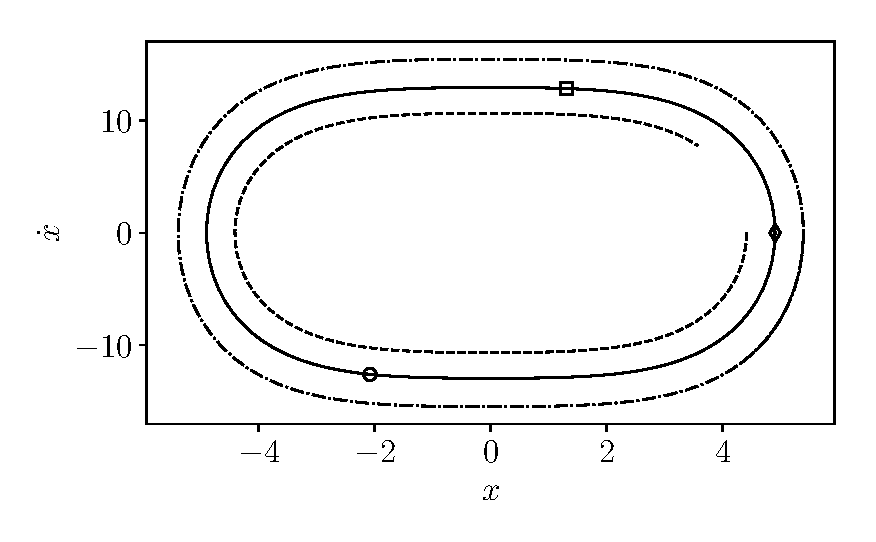
\includegraphics[width=\textwidth, height=5cm]{nnm/duff_per_space}
  \end{subfigure}
  \caption{Solution of the duffing eq. $\ddot x + x + 0.5x^3=0$ for different
    initial conditions and $T=2.0215$s. a): time series; b):
    phase space.
    Initial conditions for different line styles:
    \textemdash: [4.9009, 0];
    $---$: 0.9*[4.9009, 0];
    $-\cdot -\cdot-\cdot$: 1.1*[4.9009, 0];
    Markers represent different initial conditions for the periodic solution.
    $\diamond$: [4.9009, 0];
    $\square$: [1.308, 12.8764];
    $\circ$: [-2.0825, -12.6177]
  }
  \label{fig:sm_phase}
\end{figure}


In summary, the periodic solution is found by solving
\begin{equation}
  \label{eq:sm_bvp_problem}
  \begin{cases}
    H(\bm z_{p0}, T) = 0 \\
    h(\bm z_{p0} ) = 0
  \end{cases}
\end{equation}

The corrections to the initial guess is found by Newton-Raphson iterations. The
shooting function is expanded in a Taylor series
% around increments $\Delta \bm z_{p0}$ and $\Delta T_{p0}$

\begin{equation}
  \label{eq:sm_nr}
  \bm H(\bm z_{p0},T) +
  \frac{\p \bm H}{\p \bm z_{p0}}\bigg|_{(\bm z_{p0},T)} \Delta \bm z_{p0} +
  \frac{\p \bm H}{\p T_{p0}}\bigg|_{(\bm z_{p0},T)} \Delta T +
  + hot. = 0
  % Jeg har glemt mixede product herunder:
  %\mathcal{O}(\Delta \bm z_{p0}^2, \Delta T_{p0}^2) = 0
\end{equation}
where $hot.$ is higher order terms.


Thus the corrections are found by solving the linear equation
\begin{equation}
  \label{eq:sm_nr_sol}
  \begin{bmatrix}
    \frac{\p \bm H}{\p \bm z_{p0}}\big|_{(\bm z_{p0},T)} &
    \frac{\p \bm H}{\p T_{p0}}\big|_{(\bm z_{p0},T)} \\
    \frac{\p h}{\p \bm z_{p0}}\big|_{(\bm z_{p0},T)} &
    0
  \end{bmatrix}
  \begin{bmatrix}
    \Delta \bm z_{p0} \\
    \Delta T
  \end{bmatrix}
  =
  \begin{bmatrix}
    -\bm H(\bm z_{p0},T) \\
    -h(\bm z_{p0},T)
  \end{bmatrix}
\end{equation}
since $\bm h_{NNM}$ have the transformation $\mathbb{R^{nz+1}} \rightarrow
\mathbb{R^{nz+1}}$ the system above is over determined, ie. the matrix to
invert is not square, and is solved in a least square sense.

The state is updated as

\begin{equation}
  \label{eq:sm_nr_update}
  \bm z^{k+1}_{p0} = \bm z^k_{p0} + \Delta \bm z^k_{p0}, \quad
  T^{k+1} = T^k + \Delta T^k
\end{equation}
where $k$ is iteration number. The iteration is stopped when $\bm H = 0$ to
some tolerance. Newmark-Raphson is a local algorithm. Convergence is guarantied
when the initial guess is close to solution. Otherwise not. The initial guess
could for instance be the first linear mode and corresponding period. If the
Jacobian matrix is exact, the convergence is second order.

It should be mentioned that for some forcing parameters, where a nonlinear
system might have multiple solutions, the NR will, depending on the initial
conditions, converge towards only one of them. Methods relying on the homotopy
method or Groebner bases can be employed to find multiple solution - not that I
know anything about these methods.

\subsubsection{Sensitivity analysis}
\label{sec:sm_sens_ana}

The partial derivatives of the shooting function, used in the NR iterations, are
found as:

\begin{align}
  \label{eq:sm_jac1}
  \frac{\p \bm H}{\p T} &=
  \frac{\p \bm z(t, \bm z_0)}{\p t}\bigg|_{t=T} =
  \bm g(\bm z(T, \bm z_0)) \\
  \frac{\p \bm H}{\p \bm z_{0}} &=
  \frac{\p \bm z(t, \bm z_0)}{\p \bm z_0}\bigg|_{t=T} - \bm I
  \label{eq:sm_jac2}
\end{align}
$\p \bm H / \p T$ is a $2n$ vector. The Jacobian matrix $\p \bm H / \p \bm
z_{0}$ is $2n\times 2n$, same as the identity matrix $\bm I$.

The Jacobian matrix $\p \bm z(t,\bm z_0) / \p \bm z_{0}$, which represent the
variation of the solution $\bm z(t,\bm z_0)$ at time $t$ when the initial
conditions $\bm z_0$ are pertubated, is normally calculated in two ways. Either
by finite difference: successively pertubation of each of the $2n$ initial
condtion and integrating over the period. This is computationally expensive and
gives slower NR convergence since the Jacobi matrix is only approximate.

Instead sensitivity analysis is used. The state space formulation
\eqref{eq:sm_state} is differentiated with respect to initial conditions $\bm
z_0$

\begin{align}
  &\frac{\p}{\p \bm z_0} \left[ \dot{\bm z}(t, \bm z_0) \right] =
    \frac{\p}{\p \bm z_0} \left[ \bm g(\bm z(t, \bm z_0)) \right] \implies
    \\
  &\frac{\d}{\d t} \left[  \frac{\p \bm z(t, \bm z_0)}{\p \bm z_0} \right] =
    \frac{\p \bm g(\bm z)}{\p \bm z}\bigg|_{\bm z(t,\bm z_0)}
    \frac{\p \bm z(t, \bm z_0)}{\p \bm z_0}
    \label{eq:sm_sens}
\end{align}
with initial condition
\begin{equation}
  \label{eq:sm_sens_init}
  \frac{\bm z(0,\bm z_0)}{\bm z_0} = \bm I
\end{equation}
since $\bm z(0,\bm z_0) = \bm z_0$

Then eq. \eqref{eq:sm_sens} is integrated over $T$ to obtain the Jacobian matrix
at time $t=T$. This integration is linear and carried out at the same time as
the Newmark integration of the periodic solution. In practise the EOM
formulation eq. \eqref{eq:per_eom} is used for the sensitivity analysis. See
appendix \ref{sec:newmark_sens} for a derivation. The sensitivity analysis
requires the nonlinear forces to be smooth. If they are nonsmooth, finite
difference have to be used.

\subsubsection{Stability}
\label{sec:sm_stab}

The stability of a periodic solution is found from the Jacobian matrix evaluated
at $t=T$, called the \textit{monodromy matrix}

\begin{equation}
  \label{eq:sm_stab}
  \Phi = \frac{\p \bm z(t, \bm z_0)}{\p \bm z_0}\bigg|_{t=T}
\end{equation}
It determines whether a small initial perturbation decays or grows. The
stability is found from the eigenvalues $\sigma_i$, the Floquet multipliers. If an
Floquet multiplier is larger than one (i.e., $|\sigma_i|> 1$), the orbit is
unstable. Conversely, the periodic orbit is stable if $|\sigma_i \leq 1, \forall i$

Equivalently the Floquet exponents $\lambda$ could be used. If there is at least
one Floquet exponents with a real part larger than 0 the solution is unstable.
They are related through the relation

\begin{equation}
  \label{eq:floquet_relations}
  \sigma_i = e^{\lambda_i T}
\end{equation}

Both variants are depicted on the complex plane and either compared to the unit
circle or the imaginary axis, respectively.

\subsection{Harmonic balance}
\label{sec:harmonic_bal}

Where the shooting method finds a periodic solution by solving the system in
time domain, HB finds the periodic solution in frequency domain. The method is
described in \citet{detroux2016a}. A periodic solution to the damped and forced
EOM eq. \eqref{eq:per_eom} is sought.

As the signal $\bm x$ and forces $\bm f(\bm x, \dot{\bm x}, \omega ,t) = \bm
p(\omega, t)- \bm f_{nl}(\bm x \dot{\bm x})$ are assumed periodic, they are
approximated by Fourier series truncated to the $N_H$-th harmonic

\begin{align}
  \label{eq:hb_x_expansion}
  \bm x(t) &= \frac{\bm c^x_0}{\sqrt{2}} \sum_{k=1}^{N_h} (s^x_k \sin(k\omega t) +
          c^x_k \cos(k\omega t)) \\
  \label{eq:hb_f_expansion}
  \bm f(t) &= \frac{\bm c^f_0}{\sqrt{2}} \sum_{k=1}^{N_h} (s^f_k \sin(k\omega t) +
          c^f_k \cos(k\omega t))
\end{align}

where $\bm s_k$ and $\bm c_k$ represent the vectors of the Fourier coefficients
related to sine and cosine terms. The Fourier coefficients of the force $\bm f(t)$,
$\bm s^f_k$ and $\bm c^f_k$ depends on the Fourier coefficients of the
displacement $\bm x(t)$, $\bm s^x_k$ and $\bm c^x_k$ which are the new unknowns.
Gathering the coefficients into vectors

\begin{align}
  \label{eq:hb_coeffz}
  &\bm z =
    \begin{bmatrix}
      (\bm c^x_0)^T & (\bm s^x_1)^T & (\bm c^x_1)^T & \cdots &
      (\bm s^x_{N_H})^T & (\bm c^x_{N_H})^T
    \end{bmatrix}^T \\
  \label{eq:hb_coeffz}
  &\bm b =
    \begin{bmatrix}
      (\bm c^f_0)^T & (\bm s^f_1)^T & (\bm c^f_1)^T & \cdots &
      (\bm s^f_{N_H})^T & (\bm c^f_{N_H})^T
    \end{bmatrix}^T
\end{align}

Using a compact notion the displacement and force is written
\begin{align}
  \label{eq:hm_x_compact}
  &\bm x(t) = (\bm Q(t) \otimes \mathbb{I}_n) \bm z \\
  \label{eq:hb_y_compact}
  &\bm f(t) = (\bm Q(t) \otimes \mathbb{I}_n) \bm b
\end{align}
where $\otimes$ is the Kronecker product, $\mathbb{I}_n$ the identity matrix of
size $n$ and $\bm Q$ a vector with harmonic terms

\begin{equation}
  \label{eq:hb_Q}
  \bm Q(t) =
  \begin{bmatrix}
    \frac{1}{2} & \sin(\omega t) & \cos(\omega t) & \cdots & \sin(N_H \omega t) &
    \cos(N_H \omega t)
  \end{bmatrix}
\end{equation}

Velocities and accelerations are found using the Fourier series as
\begin{align}
  \label{eq:hb_vel}
  &\dot{\bm x} = \left( \dot{\bm Q}(t) \otimes \mathbb{I}_n \right) \bm z =
    \left( (\bm Q(t) \bm \nabla) \otimes \mathbb{I}_n \right) \bm z \\
  \label{eq:hb_acc}
  &\ddot{\bm x} = \left( \ddot{\bm Q}(t) \otimes \mathbb{I}_n \right) \bm z =
    \left( (\bm Q(t) \bm \nabla^2) \otimes \mathbb{I}_n \right) \bm z \\
\end{align}

By substituting eqs. \eqref{eq:hb_x_expansion}-\eqref{eq:hb_f_expansion} and
\eqref{eq:hb_vel}-\eqref{eq:hb_acc} into the EOM \eqref{eq:per_eom} and using a
galerkin procedure, one ends up with the equations of motion in frequency
domain (see appendix \ref{sec:hb_appendix} for more details on the derivation
and definition of $\bm \nabla$)

\begin{equation}
  \label{eq:hb_feom}
  (\bm \nabla^2 \otimes \bm M)\bm z + (\bm \nabla \otimes \bm C)\bm z +
  (\mathbb{I}_{2N_H} \otimes \bm K)\bm z =
  (\mathbb{I}_{2N_H} \otimes \mathbb{I}_n )\bm b
\end{equation}
or in more compact form

\begin{equation}
  \label{eq:hb_feom_compact}
  \bm H(\bm z, \omega) = \bm A(\omega) \bm z - \bm b(\bm z) = \bm 0
\end{equation}
where $\bm A$ describes the linear dynamics

\begin{equation}
  \label{eq:hb_A}
  \bm A = \bm \nabla^2 \otimes \bm M + \bm \nabla \otimes \bm C +
  \mathbb{I}_{2N_H} \otimes \bm K
\end{equation}

If $z^*$ is a solution of \eqref{eq:hb_feom_compact}, then the time signal $x^*$
constructed from $z^*$ is periodic and satisfies the eom \eqref{eq:per_eom}. As
with the shooting function, eq. \eqref{eq:hb_feom_compact} is nonlinear (due to
$\bm b$ dependence on $\bm z$) and have to be solved iteratively by
Newton-Rahpson iterations. It should however be noted that $\bm H(\bm z,
\omega)$ is an (nonlinear) algebraic equation, ie there is no need for
integration.

\begin{equation}
  \label{eq:hb_nr}
  \bm z^{(k+1)} = \bm z^{(j)} -
  \frac{\bm H(\bm z, \omega)}{\bm H_{\bm z}(\bm z, \omega)}
\end{equation}


\subsubsection{Expression of nonlinear terms and Jacobian matrix}
\label{sec:hb_exp_nonlin_jac}

Solution of eq \eqref{eq:hb_nr} requires calculation of $\bm H$ and of the
Jacobian matrix $\bm H_{\bm z}$, which in turn requires calculation of $\bm b$
and its derivatives.

It is not known how the Fourier coefficients in $\bm b$ relates to the
coefficients in $\bm z$, ie. it is not possible to directly calculate $\bm b(\bm
z)$ due to $\bm f_{nl}$ depends on $x$. Instead a technique called the
\textit{alternating frequency-time domain}(AFT) method is used. Here $\bm b$ is
calculated through successive Fourier transformations as shown in the graph below.

\begin{center}
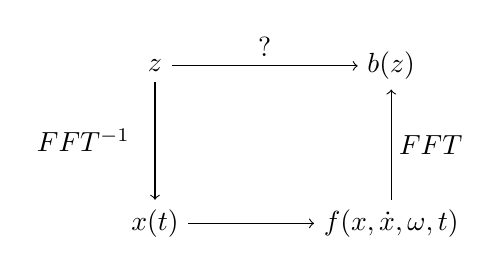
\begin{tikzpicture}[node distance=1.5cm]
  % nodes
  \node (A) at (0, 2) {$\bm z$};
  \node (B) at (0, 0) {$\bm x(t)$};
  \node (C) at (3, 0) {$\bm f(\bm x,\dot{\bm x},\omega, t)$};
  \node (D) at (3, 2) {$\bm b(\bm z)$};
  % arrows
  \draw [->]
  (A) edge node[anchor=center, text width=3.0cm] {$FFT^{-1}$} (B)
  (B) edge (C)
  (C) edge  node[anchor=center, text width=-0.2cm] {$FFT$} (D)
  (A) edge  node[anchor=center, above] {?} (D);
\end{tikzpicture}
\captionof{figure}{Graphical representation of the alternating frequency-time
  domain (AFT) method}
\end{center}

$\bm x$ is calculated from the Fourier coefficients in $\bm z$, then the
nonlinear (and external) forces $\bm f$ are evaluated in time domain and $\bm b$
is found as the Fourier coefficients of $\bm f$.

The Jacobian matrix is given by
\begin{equation}
  \label{eq:hb_jac1}
    \bm H_{\bm z} = \frac{\p \bm H}{\p \bm z} = \bm A - \frac{\p \bm b}{\p \bm z}
\end{equation}
where the hard part is to compute $\bm b_{\bm z}$. The method for calculating
the Jacobian matrix follows the AFT method as well. To do that, the inverse
Fourier transform is rewritten as the linear operator $\Gamma(\omega)$

\begin{equation}
  \label{eq:hb_gamma}
  \begin{aligned}
    \bm \Gamma(\omega) =
    \left[
  \begin{matrix}
    \mathbb{I}_n \otimes
    \begin{bmatrix}
      1/\sqrt{2} \\ 1/\sqrt{2} \\ \vdots \\ 1/\sqrt{2}
    \end{bmatrix} &
    \mathbb{I}_n \otimes
    \begin{bmatrix}
      \sin(\omega t_1) \\ \sin(\omega t_2) \\ \vdots \\ \sin(\omega t_{t_N})
    \end{bmatrix} &
    \mathbb{I}_n \otimes
    \begin{bmatrix}
      \cos(\omega t_1) \\ \cos(\omega t_2) \\ \vdots \\ \cos(\omega t_{t_N})
    \end{bmatrix}&
        \cdots
  \end{matrix}
\right. \\
\left.
  \begin{matrix}
    \mathbb{I}_n \otimes
    \begin{bmatrix}
      \sin(N_H\omega t_{}) \\ \sin(N_H\omega t_2) \\ \vdots \\ \sin(N_H\omega t_{t_N})
    \end{bmatrix} &
    \mathbb{I}_n \otimes
    \begin{bmatrix}
      \cos(N_H\omega t_{}) \\ \cos(N_H\omega t_2) \\ \vdots \\ \cos(N_H\omega t_{t_N})
    \end{bmatrix}
  \end{matrix}
\right]
\end{aligned}
\end{equation}

which is used on the concatenated time series
\begin{equation}
  \label{eq:hb_time_series}
  \begin{aligned}
    \tilde{\bm x} =
    \begin{bmatrix}
      x_1(t_1) & \cdots & x_1(t_N) & \cdots & x_n(t_1) & \cdots & x_n(t_N)
    \end{bmatrix}^T\\
    \tilde{\bm f} =
    \begin{bmatrix}
      f_1(t_1) & \cdots & f_1(t_N) & \cdots & f_n(t_1) & \cdots & f_n(t_N)
    \end{bmatrix}^T
  \end{aligned}
\end{equation}

Thus the inverse and direct Fourier transform are written
\begin{equation}
  \label{eq:hb_four_transform}
    \tilde{\bm x} = \bm \Gamma(\omega) \bm z, \quad
    \bm z =( \bm \Gamma(\omega))^+ \tilde{\bm x}
\end{equation}
where $()^+$ is the Moore-Penrose pseduinverse which is needed since $\Gamma$ is
not square. (In implementing, one would use a least-square iterative solver
instead of calculating the pseduinverse, since the former is faster. Both
methods gives a solution which have a minimum norm in some sense.)

The Fourier coefficients of the external and nonlinear forces are then
\begin{equation}
  \label{eq:hb_b_coeff}
  \bm b(\bm z) = ( \bm \Gamma(\omega))^+ \tilde{\bm f}
\end{equation}
and the Jacobian is computed as
\begin{equation}
  \label{eq:hb_jac}
  \bm H_{\bm z} = \bm A - \frac{\p \bm b}{\p \bm z} =
  \bm A -
  \frac{\p\bm b}{\p \tilde{\bm f}}
  \frac{\p \tilde{\bm f}}{\p \tilde{\bm x}}
  \frac{\p \tilde{\bm x}}{\p \bm z} =
  \bm A - \bm \Gamma^+ \frac{\p \tilde{\bm f}}{\p \tilde{\bm x}} \bm \Gamma
\end{equation}

It should be noted that the concatenated time series vectors $\tilde{\bm x}$ and
$\tilde{\bm f}$ are newer used. They are only used in the derivation for the
expression for the Jacobian. Only the Fourier operator $\bm \Gamma$ and
extracted Fourier coefficients $\bm x$ are used.


\subsubsection{Stability}
\label{sec:hb_stab}

Unlike the shooting method (or general time domain methods), the monodromy
matrix is not readily available as a byproduct since there is no time
integration. Instead for frequency methods, \textit{Hills method} is used to
approximate the Floquet exponents by solving a quadratic eigenvalue problem
whose components are obtained as byproduct of the HB method.

Perturbing a periodic solution by an exponential decay
\begin{equation}
  \label{eq:hb_pert}
  \bm p(t) = \bm x(t) + e^{\lambda t}\bm s(t)
\end{equation}
and inserting this into the eom eq. \eqref{eq:per_eom} it is shown in appendix
\ref{sec:hb_stab_appendix} that the quadratic eigenvalue problem is found as

\begin{equation}
  \label{eq:hb_quad_eigen}
  \bm \Delta_2 \bm \lambda^2 + \bm \Delta_1 \bm \lambda + \bm H_{\bm z} = \bm 0
\end{equation}
where $\bm \Delta$ are matrices describing the linear dynamics similar to $\bm
A$ in eq. \eqref{eq:hb_A} and $\lambda$ are Hills coefficients.

The quadratic eigenvalue problem is rewritten to a linear eigenvalue problem of
double size

\begin{equation}
  \label{eq:hb_double_eigen}
  \bm B_1 - \gamma \bm B_2 = \bm 0
\end{equation}
where

\begin{equation}
  \label{eq:hb_stab_B12}
  \bm B_1 =
  \begin{bmatrix}
    \bm \Delta B_1 & \bm H_{\bm z} \\
    -\mathbb{I}    & \bm 0
  \end{bmatrix}, \quad
  \bm B_2 = -
  \begin{bmatrix}
    \bm \Delta_2   & \bm 0 \\
    \bm 0          & \mathbb{I}
  \end{bmatrix}
\end{equation}

The coefficients $\bm \lambda$ are found as the eigenvalues of the $(2N_H+1)2n
\times (2N_H+1)2n$ matrix

\begin{equation}
  \label{eq:hb_B}
  \bm B = \bm B^{-1}_2 \bm B_1 =
  \begin{bmatrix}
    -\bm \Delta^{-1}_2 \bm\Delta_1 & -\bm \Delta^{-1}_2 \bm H_{\bm z} \\
    \mathbb{I}                    & \bm 0
  \end{bmatrix}
\end{equation}
or from the generalised eigenvalueproblem eq. \eqref{eq:hb_stab_B12}.

Only $2n$ eigenvalues approximate the Floquet exponents $\tilde{\bm \lambda}$,
the rest are spurious. The real ones are the $2n$ values with smallest imaginary
magnitude.

The diagonal matrix
\begin{equation}
  \label{eq:hb_B_tilde}
  \tilde{\bm B} =
  \begin{bmatrix}
    \tilde \lambda_1 \\
    & \ddots \\
    & & \tilde \lambda_{2n}
  \end{bmatrix}
\end{equation}
gathers the Floquet exponents identified from the $(2_{N_H} + 1)2n$ Hill's
coefficients. Besides stability, they are used for detecting bifurcations in
section \ref{sec:detecting_bifs}.

\subsubsection{Example}
\label{sec:hb_example}

Figure \ref{fig:hb_duffing_periodic} shows the periodic of the coupled duffing
Duffing system. Although the excitation is pure sine, the response contains
multiple harmonics due to nonlinearity. The normalized harmonic components are
found as

\begin{equation}
  \label{eq:hb_normal_coeff}
  \begin{aligned}
    \sigma_i = \frac{\phi_i}{\sum_{k=0}^{N_H} \phi_i}, \quad (i=0,\cdots, N_H) \\
    \phi_0 = \frac{c_0^x}{\sqrt{2}}, \quad \phi_i = \sqrt{(s^x_i) + (c^x_i)^2}
  \end{aligned}
\end{equation}

% \begin{figure}[!ht]
%   \centering
%   \begin{subfigure}[b]{0.6\textwidth}
%       \setlength\figureheight{6cm}
%       \setlength\figurewidth{\textwidth}
%       \InputIfFileExists{fig/2dof_duffing/hb_per.tex}{}
%       {\textbf{!! Missing graphics !!}}
%   \end{subfigure}
%   ~~~
%   \begin{subfigure}[b]{0.36\textwidth}
%       \setlength\figureheight{6cm}
%       \setlength\figurewidth{\textwidth}
%       \InputIfFileExists{fig/2dof_duffing/hb_har.tex}{}
%       {\textbf{!! Missing graphics !!}}
%   \end{subfigure}
%   \caption{Periodic solution of the coupled Duffing system for $f=2$,
%     $\omega=1.2$ and $N_H=5$.
%     (a): Time series; (b): Normalized harmonic components of $x_1$.}
%   \label{fig:hb_duffing_periodic}
% \end{figure}

\begin{figure}[!ht]
  \centering
  \begin{subfigure}[b]{0.6\textwidth}
    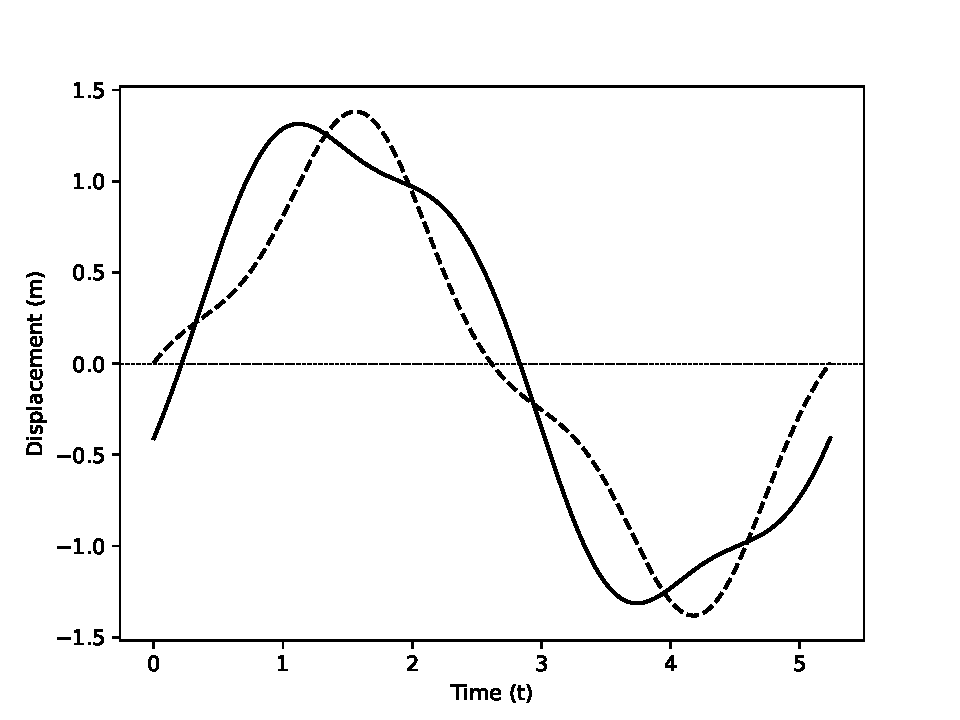
\includegraphics[width=\linewidth, height=6cm]{2dof_duffing/hb_per.tikz}
    \caption{}
  \end{subfigure}
  ~
  \begin{subfigure}[b]{0.36\textwidth}
    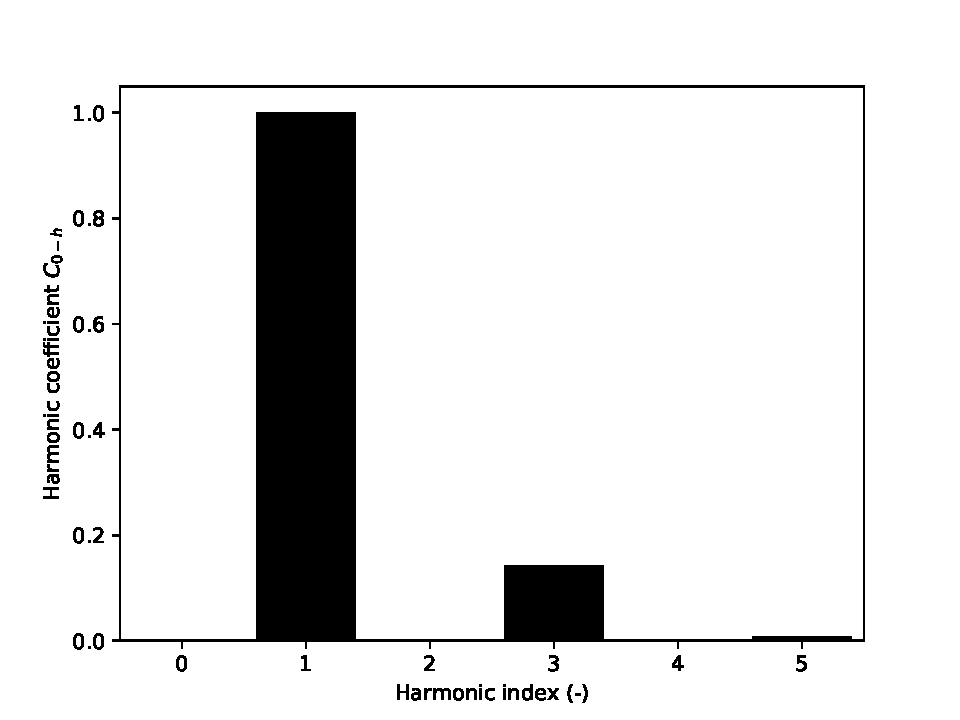
\includegraphics[width=\linewidth, height=6cm]{2dof_duffing/hb_har.tikz}
    \caption{}
  \end{subfigure}
    \caption{Periodic solution of the coupled Duffing system for $f=2$,
    $\omega=1.2$ and $N_H=5$.
    (a): Time series; (b): Normalized harmonic components of $x_1$.}
  \label{fig:hb_duffing_periodic}
\end{figure}
\FloatBarrier

\subsection{Summary}
\label{sec:per_summary}

Periodic solutions of nonlinear structures can be computed with
time-domain(shooting method) and frequency-domain(harmonic balance) methods. The
main difference is in the implementation complexity, computional complexity and
accuracy. Both methods can be used together with continuation and are natural
integrated with stability analysis.

Summarising the shooting method
\begin{multicols}{2}
  Pro
  \begin{itemize}
  \item Accurate
  \item Higher harmonics represented
  \end{itemize}
  \columnbreak
  Cons
  \begin{itemize}
  \item Many time integrations
  \item Slow for larger systems
  \end{itemize}
\end{multicols}
If the shooting method should be used for damped and forced motion, only the
state space formulation have to be changed. See appendix
\ref{sec:shooting_appendix} for the few changes.

Summarising the harmonic balance method
\begin{multicols}{2}
  Pro
  \begin{itemize}
  \item Fast
  \item Harmonic coefficients available
  \item Can be used for filtering
  \end{itemize}
  \columnbreak
  Cons
  \begin{itemize}
  \item Less accurate
  \item High number of harmonic might be necessary. Need to check the
    contribution from last harmonics to ensure enough is included.
  \end{itemize}
\end{multicols}


Stability of a periodic solution can be assessed through  their Floquet
multipliers or exponents. When the Shooting method is used, they are found from
the monodromy matrix. When \gls{hb} is used, they are found from Hills matrix.


%%% Local Variables:
%%% mode: latex
%%% TeX-master: "../../report"
%%% End:
